\documentclass{article}

\usepackage[francais]{babel}
\usepackage[T1]{fontenc}
\usepackage{moreverb}       % verbatim with tab

\usepackage{wrapfig}
\usepackage{graphicx}
\usepackage{geometry}
\geometry{hmargin=2.5cm}
\usepackage{amsmath}
\usepackage{siunitx}

\usepackage{graphicx}
\usepackage{subcaption}
\usepackage{float}
\usepackage{hyperref}
\usepackage{setspace}
\usepackage{xcolor}
\usepackage{pdfpages}
\usepackage{enumitem}
\usepackage{lscape}

\usepackage{fancyhdr}       % en-têtes
\usepackage{lastpage}       % numéro de dernière page

\title{}

\title{Programmation procédurale\bigbreak \bigbreak
    \large Dossier 2\bigbreak
    \normalsize Transformations d’images bitmap\bigbreak}
\date{2020 -- 2021}
\author{Laura Binacchi}

\pagestyle{fancy}
\renewcommand\headrulewidth{1pt}
\fancyhead[L]{Laura Binacchi}
\fancyhead[C]{Programmation procédurale}
\fancyhead[R]{\today}


\begin{document}
    \pagenumbering{gobble}
    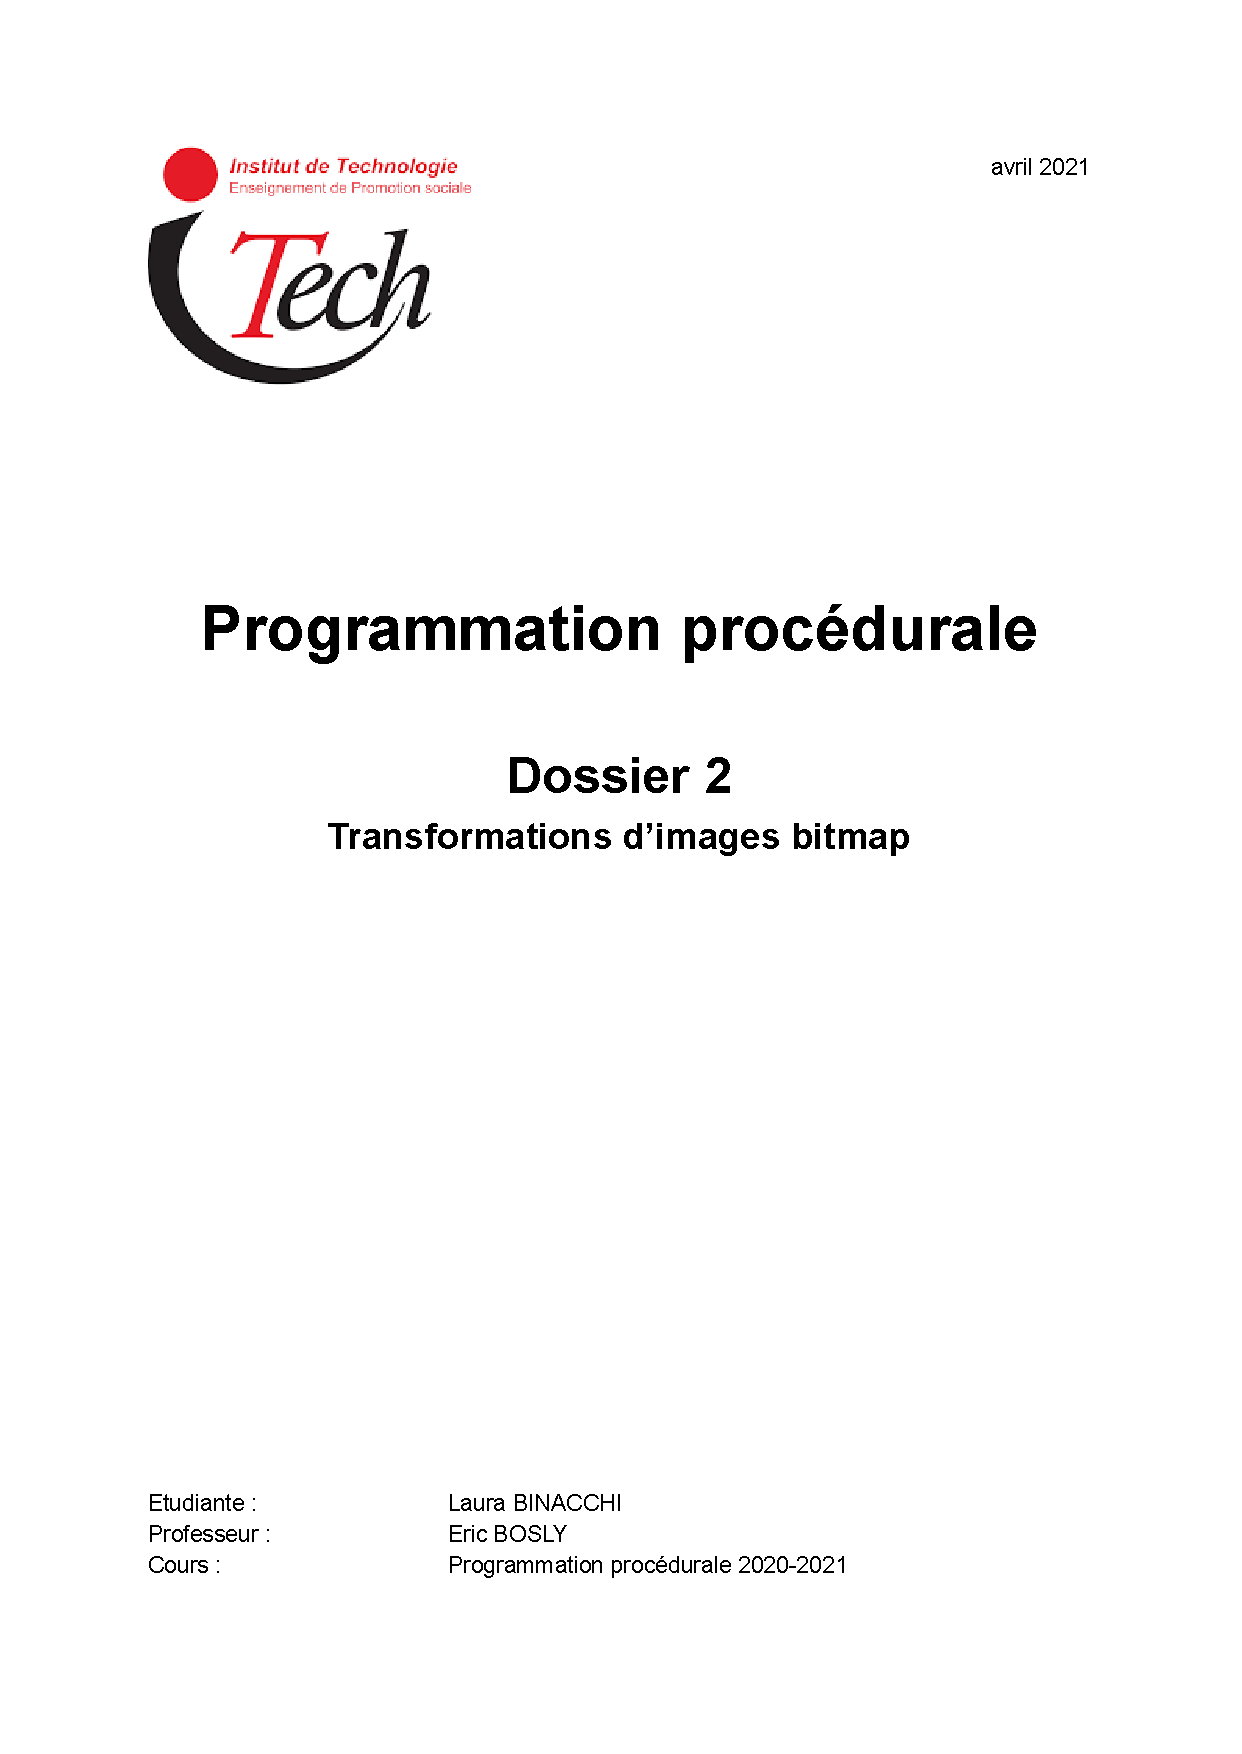
\includepdf[pages={1}]{pdg}
    \newpage
    \tableofcontents
    \newpage
    \pagenumbering{arabic}

    \section{Cahier des charges}
    \paragraph{}
    On demande d’écrire un programme en C qui permet de générer une série de fichiers image au format .bmp 24 bits. Ces images seront  obtenues par application de filtres décrits ci-dessous à des images existantes. Le programme fonctionnera en 2D, le but de l’exercice n’est pas artistique mais bien de concevoir et implémenter des effets graphiques faisant appel à plusieurs images. Le programme sera décomposé en blocs fonctionnels cohérents,fera appel à l’allocation dynamique des matrices utilisées et sera écrit de manière lisible et bien documentée. Il utilisera au maximum les notions de programmation vues au cours, spécialement les structures, les fichiers binaires,les boucles imbriquées complexes à indices multiples et variables.

    \paragraph{}
    Ce programme sera purement «batch», aucune interactivité n’est demandée. Le programme principal appellera un ensemble de routines de tests générant les images demandées, mais aussi testant de manière systématique les fonctions primitives nécessaires.

    \subsection{Filtre 1: pavage d'images}
    \paragraph{}
    Une image est divisée en pavés carrés. Dans une première version, ces pavés seront de couleur constante, égale à la couleur moyenne de la portion d’image. Ensuite le pavé sera obtenu par redimensionnement de l’image et recolorisation afin de rendre l’aspect global de l’image.

    \subsection{Filtre 2: images en donut}
    \paragraph{}
    Une transformation de coordonnées entre des coordonnées cartésiennes et polaires permet de représenter l’image sous forme d’un donut.
    
    \paragraph{}
    Ces deux effets sont évidement combinables...


    \newpage
    \section{Description du programme}
    \subsection{Fonctions utilitaires}
    \paragraph{}
    Avant l'implémentation des filtres, il est nécessaire d'implémenter des fonctions utilitaires permettant de manipuler des fichiers bitmap. Ces fonctions sont implémentées dans le fichier \emph{bmp\_file.c}.


    \subsubsection{Chargement d'un fichier bitmap}
    \paragraph{}
    La fonction \texttt{load\_bmp3} permet de charger une image bitmap dans la mémoire RAM du programme.
    
    \paragraph{}
    Cette fonction doit charger en deux temps l'identifiant du fichier (les caractères \texttt{BM}) et le reste des données afin d'éviter un décalage dû au padding ajouté par le compilateur. En effet, le compilateur ajoute de l'espace pour que les champs soient alignées sur quatre bytes, ce qui ne pose de problème pour ce programme que dans le cas de la lecture des informations du fichier.
    
    \paragraph{}
    Le chargement de l'image dans la matrice de pixels tient également compte du padding du fichier bitmap : chaque ligne est composée d'un certain nombre de pixels de trois bytes mais la taille de la ligne entière est un multiple de quatre bytes.
    
    \paragraph{}
    Dès que l'image n'est plus utilisée, la fonction \texttt{free\_bmp3} doit être appelée pour libérer la mémoire allouée à la matrice de pixels de l'image.

    \subsubsection{Affichage des métadonnées du fichier}
    \paragraph{}
    La fonction \texttt{print\_bmp3\_info} permet d'afficher les métadonnées d'une image chargée en mémoire. Cette fonction permet de vérifier la conformité des données chargées avec l'image source. Elle permet également de vérifier l'intégrité des données chargées avec celles du fichier bitmap en ouvrant ce fichier dans un éditeur hexadécimal.

    \subsubsection{Écriture d'une image}
    \paragraph{}
    La fonction \texttt{write\_bmp3} écrit une image en mémoire dans un nouveau fichier (ou en écrasant le fichier existant s'il y en avait un). Comme la fonction de chargement, elle tient compte du padding des lignes du fichier bitmap.

    \subsubsection{Création d'une image}
    \paragraph{}
    La fonction \texttt{create\_bmp3} permet de créer une nouvelle image aux dimensions souhaitées. Par défaut, l'image est noire car sa matrice de pixels est initialisée à \texttt{0}. Il est possible de la remplir avec une autre couleur en appelant la fonction \texttt{fill\_bmp3}.


    \newpage
    \subsection{Pavage d'images}
    \paragraph{}
    Le pavage d'images est implémenté dans le fichier \emph{mosaic\_filter.c}. Ce filtre utilise la fonction utilitaire \texttt{reduce} qui permet, d'une part, de générer une image réduite contenant les couleurs moyennes des tuiles de l'image filtrée et, d'autre part, de générer l'image réduite qui sera insérée dans la tuile.

    \paragraph{}
    


    \subsection{Images en donut}




    \newpage
    \section{Tests}
    \paragraph{}
    Les tests sont implémentés dans le dossier \emph{tests} sous forme de routines appelant les différentes fonctions utilisées par le programme. Ils sont compilés en fichiers exécutables par un \emph{Makefile} généré par \emph{cmake}. La commande \texttt{cmake ..}\footnote{Pour ajouter des informations sur le code source lors du développement, j'utilise la commande \texttt{cmake -DCMAKE\_C\_FLAGS=-g ..} qui permet de remonter les erreurs plus facilement avec \emph{gdb}. Pour la version finale, j'utilise la commande \texttt{cmake -DCMAKE\_BUILD\_TYPE=Release ..}} lancée depuis le répertoire \emph{build} génère le \emph{Makefile}. La commande \texttt{make} lancée depuis ce même répertoire génère les différents exécutables.


    \subsection{Chargement d'une image}
    \paragraph{}
    Le chargement d'une image en mémoire RAM est testé dans le fichier \emph{test\_load.c}. Il teste le chargement en mémoire RAM des images de test placées dans le répertoire \emph{images} et affiche les données du header pour vérifier le chargement correct de celui-ci. Ces informations permettent notamment de vérifier que les hauteurs et largeurs en pixels des images et les tailles en bytes correspondent bien aux données des images testées.

    \subsection{Copie d'une image}
    \paragraph{}
    Le test de copie d'image implémenté dans le fichier \emph{test\_copy.c} permet de tester la fonction d'écriture d'une image bitmap en mémoire dans un fichier bitmap. Il permet également de vérifier l'intégrité des données chargées dans la matrice de pixels. Les images crées sont comparées aux images d'origine avec la commande \texttt{diff}.


    \subsection{Création d'une image}
    \paragraph{}
    La création d'une nouvelle image est testée par le fichier \emph{test\_create.c}. Ce test vérifie que la fonction de création crée bien une image noire (la matrice de pixels est initialisée à \texttt{0}) aux dimensions demandées. Il crée des images de largeur variables dont le modulo \texttt{4} est égal à \texttt{0}, \texttt{1}, \texttt{2} et \texttt{3} pour vérifier que l'écriture de l'image gère correctement le padding des lignes. Il permet également de tester la fonction de remplissage d'une matrice de pixels avec une couleur donnée.

    \subsection{Réduction d'une image}
    \paragraph{}
    La fonction utilitaire de réduction d'une image utilisée pour le filtre de pavage est testée dans les fichiers \emph{test\_reduction.c} et \emph{test\_tile.c} qui testent les deux manières dont la fonction sera utilisée par le filtre. Le fichier \emph{test\_reduction.c} teste égalemetn les cas d'erreurs de la fonction de réduction.

    \paragraph{}
    Le test de réduction génère une image réduite d'un facteur donné. Chacun de ses pixels est initialisé avec la couleur moyenne de l'ensemble des pixels de l'image source qui sont réduits. Les réductions crées à partir des moyennes de couleurs sont plus lisible (i.e. plus proche de l'image d'origine) que les réductions ne reprenant qu'un pixel sur \texttt{x} de l'image d'origine. Cet effet est particulièrement visible pour le fichier \emph{landscape1.bmp} où les bleus sont atténués mais ne sont pas perdus.

    \paragraph{}
    Le test de création d'une tuile génère une tuile de taille de donnée et non plus de facteur donné. La tuile à insérer dasn l'image pavée sera toujours carrée. Ce test permet de vérifier le bon fonctionnement des offsets : les tuiles sont bien générées à partir du centre de l'image et pas des bords.



    \subsection{Valgrind}
    \paragraph{}
    Tous les exécutables ont été testés avec \emph{valgrind} pour vérifier que tous les espaces de mémoire alloués lors de l'exécution du programme sont bien libérés. Ces tests sont effectuées avec la commande \texttt{valgrind --leak-check=full -s ./test}\footnote{\texttt{leak-check=full} pour avoir des détails sur les fuites mémoires et \texttt{-s} pour avoir des détails sur les erreurs} où \texttt{test} est le nom de l'exécutable à tester.

    \paragraph{}
    Ces tests m'ont permis de rester attentive à toujours libérer les espaces mémoire alloués aux matrices de pixels.



    \newpage
    \section{Problèmes rencontrés}

    
\end{document}
